\paragraph{QuizziPedia::Front-End::ModelViews::PasswordForgotModelView}
	
	\label{QuizziPedia::Front-End::ModelViews::PasswordForgotModelView}
	
	\begin{figure}[ht]
		\centering
		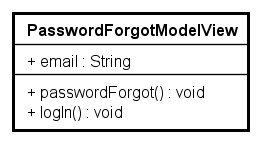
\includegraphics[scale=0.8,keepaspectratio]{UML/Classi/Front-End/QuizziPedia_Front-end_ModelView_PasswordForgotModelView.png}
		\caption{QuizziPedia::Front-End::ModelViews::PasswordForgotModelView}
	\end{figure} \FloatBarrier
	
	\begin{itemize}
		\item \textbf{Descrizione}: classe di tipo modelview la cui istanziazione è contenuta all'interno della variabile di ambiente \$scope di \textit{Angular.js\ped{G}}. All'interno di essa sono presenti le variabili e i metodi necessari per il \textit{Two-Way Data-Binding\ped{G}} tra la view \texttt{PasswordForgotView} e il controller \texttt{PasswordForgotController};
		\item \textbf{Utilizzo}: viene utilizzata per effettuare il \textit{Two-Way Data-Binding\ped{G}} tra la view \texttt{PasswordForgotView} e il controller \texttt{PasswordForgotController} rendendo disponibili variabili e metodi;
		\item \textbf{Relazioni con altre classi}: 
		\begin{itemize}
			\item \textit{OUT} \texttt{PasswordForgotView}: view contenente le form necessarie per il recupero della password dimenti- cata; 
			\item \textit{OUT} \texttt{PasswordForgotController}: questa classe permette di gestire il ripristino della password dimenticata;
		\end{itemize}
		\item \textbf{Attributi}: 
		\begin{itemize}
			\item \texttt{+ email: String} \\ Campo dati contenente l'email per il recupero password;
		\end{itemize}
		\item \textbf{Metodi}: 
		\begin{itemize}
			\item \texttt{+} \texttt{passwordForgot(email: String): void} \\
			Metodo che richiama il metodo \texttt{passwordForgot} del service \texttt{AuthService} passandogli il parametro \texttt{email}. Nel caso di buona riuscita dell'operazione, viene mostrato un messaggio di successo il cui corpo contiene anche un bottone per effettuare il redirect alla pagina di login. Nel caso in cui invece avvenga un errore, viene mostrato a video il messaggio di errore;
			\item \texttt{+} \texttt{logIn(): void} \\
			Metodo che gestisce l’evento click sul pulsante di login. Effettua il redirect alla pagina di login;
		\end{itemize}
	\end{itemize}
	
	